\doublespacing
%% ------------------------------------------------------------------------- %%
\chapter{Bancada geradora de Aeross\'{o}is}
\label{cap:bancada}

O processo de gera\c{c}\~{a}o de aeross\'{o}is inicia-se em um compressor com sa\'{\i}da de ar filtrado. Em seguida, este ar filtrado passa por uma armadilha de \'{a}gua. Nesse ponto, o ar pressurizado, filtrado e seco \'{e} injetado no atomizador TSI3076 que esta acoplado a um reservat\'{o}rio, contendo uma solu\c{c}\~{a}o de sulfato de am\^{o}nia (NH$_4$)$_2$SO$_4$. Outras subst\^{a}ncias higrosc\'{o}picas podem ser utilizadas como por exemplo nitrato de am\^{o}nia NH$_4$NO$_3$, cloreto de s\'{o}dio NaCl e etc. Na sa\'{\i}da deste atomizador, tem-se os aeross\'{o}is propriamente dito, embora polidisperssivo e com uma umidade muito alta. A remo\c{c}\~{a}o da umidade \'{e} feita por um secador a base de silicagel.

Como o processo de condensa\c{c}\~{a}o do vapor de \'{a}gua \'{e} altamente dependente do tamanho do aerossol, ou seja , do tamanho do n\'{u}cleo de condensa\c{c}\~{a}o, exige-se um controle deste par\^{a}metro. Isto \'{e}, exige-se que o aerossol seja monodispersivo. Para tal, utiliza-se na sa\'{\i}da do secador um classificador eletrost\'{a}tico, que no caso \'{e} o TSI3080. Por fim, a medida da concentra\c{c}\~{a}o das part\'{\i}culas \'{e} feita por um contador de part\'{\i}culas condens\'{a}veis (CPC), no caso o TSI3025A.

O contador de part\'{\i}culas condens\'{a}veis  TSI3025A \'{e} capaz de medir aeross\'{o}is com um di\^{a}metro de 3nm at\'{e} 3$\mu$m numa faixa de concentra\c{c}\~{a}o  de 0 at\'{e} 9,99$\cdot$10$^{4}$ part\'{\i}culas / cm$^{3}$. Em condi\c{c}\~{o}es normais, seu sensor de part\'{\i}culas opera em uma atmosfera saturada de Butanol-1.  Essa caracter\'{\i}stica o torna sens\'{\i}vel,  n\~{a}o apenas aos aeross\'{o}is respons\'{a}veis pela forma\c{c}\~{a}o das nuvens e das chuvas, mas a qualquer aerossol. Por essa raz\~{a}o, no processo de compara\c{c}\~{a}o, normalmente se utiliza apenas aeross\'{o}is higrosc\'{o}picos (como por exemplo o sulfato de am\^{o}nia, nitrato de am\^{o}nia ou cloreto de s\'{o}dio) que s\~{a}o capazes de sensibilizar tanto o CCNC-SDCC quanto o CPC TSI3025A.


\begin{figure}[hbt]
\begin{center}
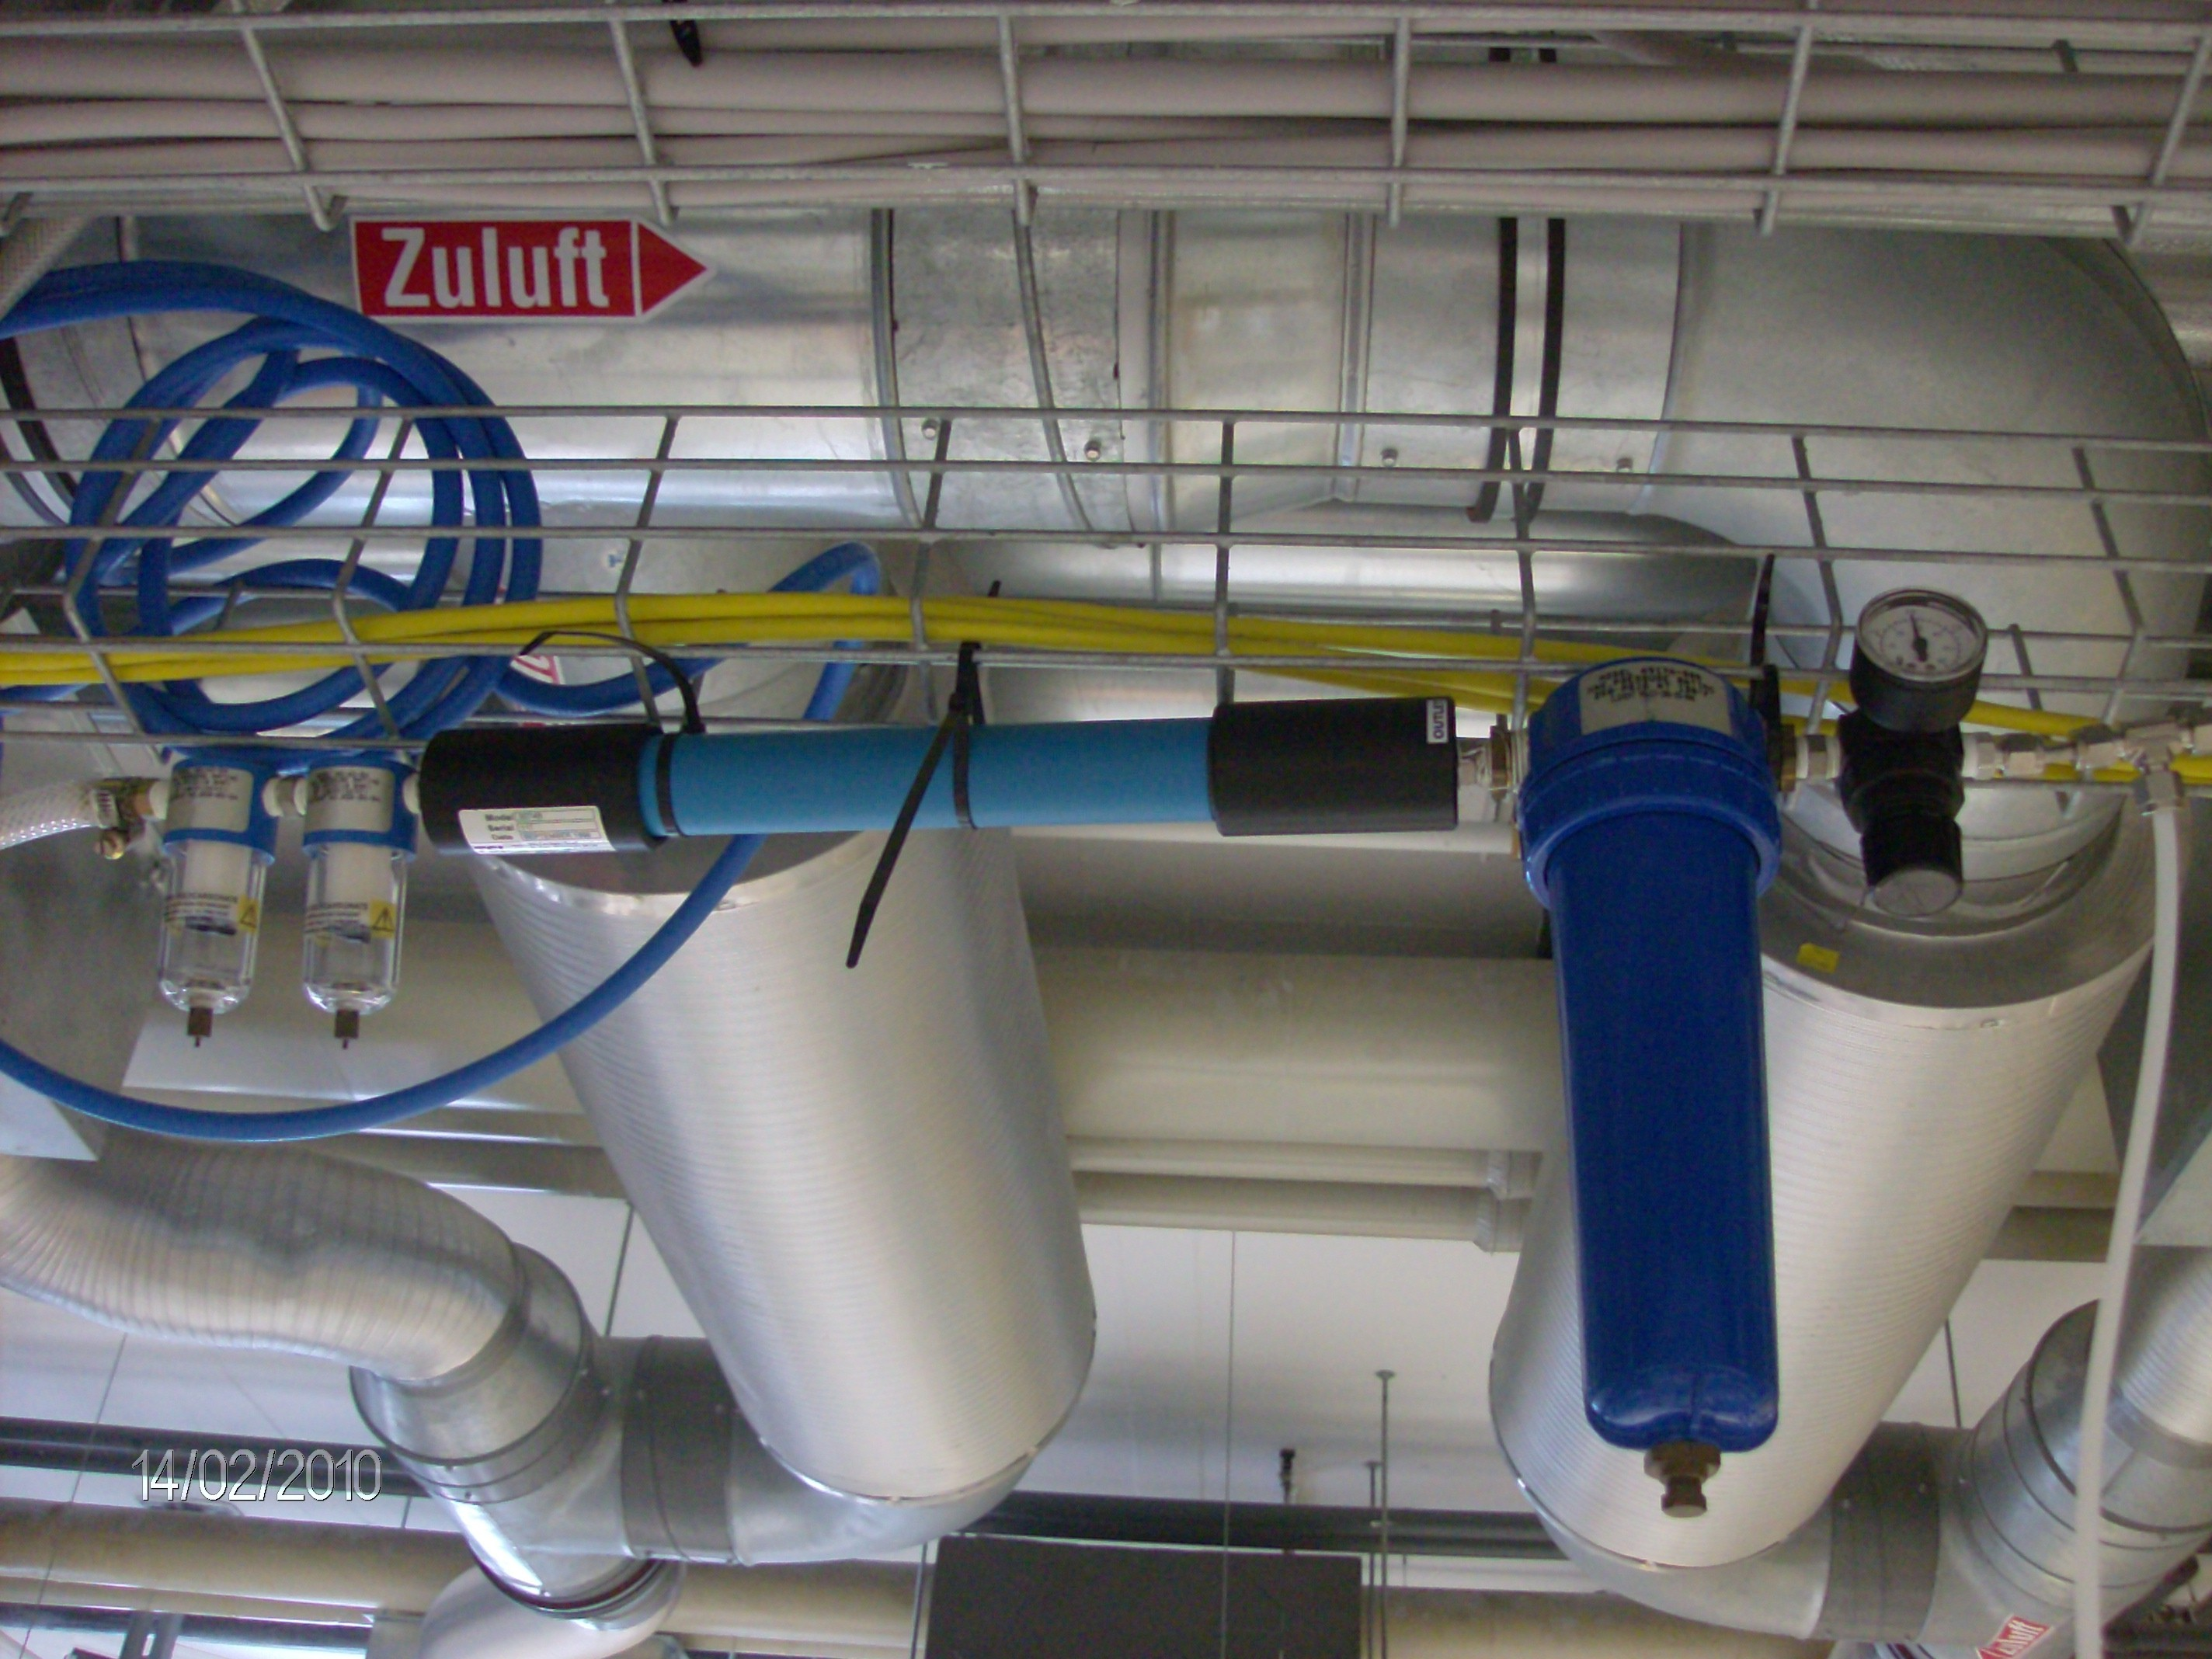
\includegraphics[scale=0.1]{eps/TSI3074FILTRO.eps}\\
\end{center}
\caption{\label{TSI3074FILTRO}\hspace{-0.1em} filtro para remo\c{c}\~{a}o de gotas de \'{o}leo, \'{a}gua e particulados (TSI3074B). }
\end{figure}

\begin{figure}[hbt]
\begin{center}
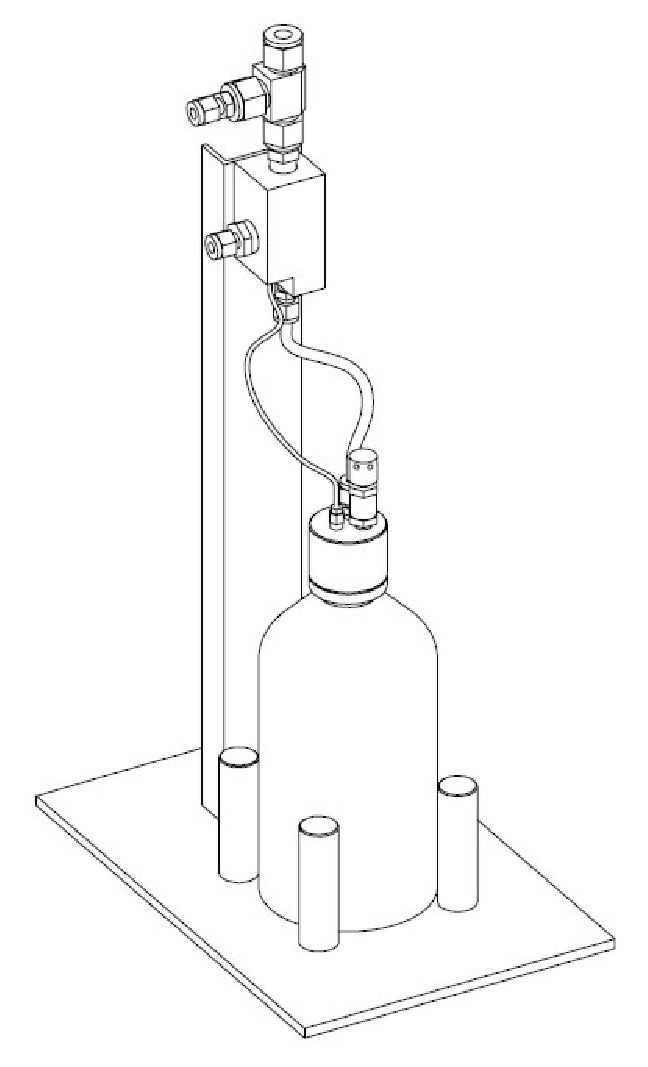
\includegraphics[scale=0.5]{eps/TSI3076ATOMIZADOR.eps}\\
\end{center}
\caption{\label{TSI3074FILTRO}\hspace{-0.1em} diagrama esquem\'{a}tico do atomizador (TSI3076).}
\end{figure}

\begin{figure}[hbt]
\begin{center}
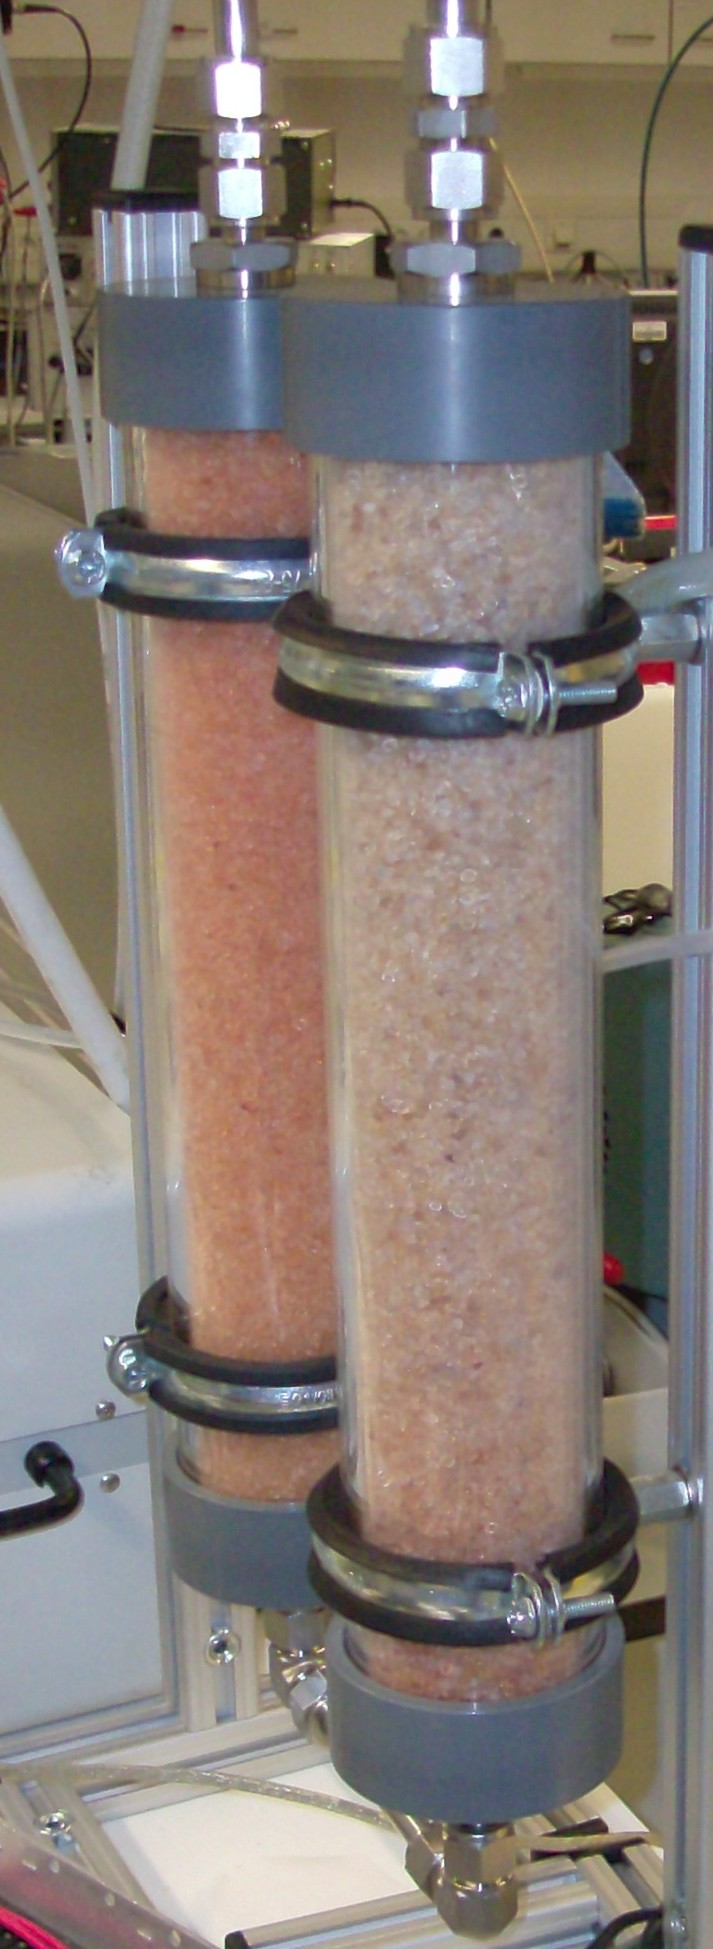
\includegraphics[scale=0.1]{eps/TSI3062SECADOR.eps}\\
\end{center}
\caption{\label{TSI3062SECADOR}\hspace{-0.1em} secador (TSI3062).}
\end{figure}



\begin{figure}[hbt]
\begin{center}
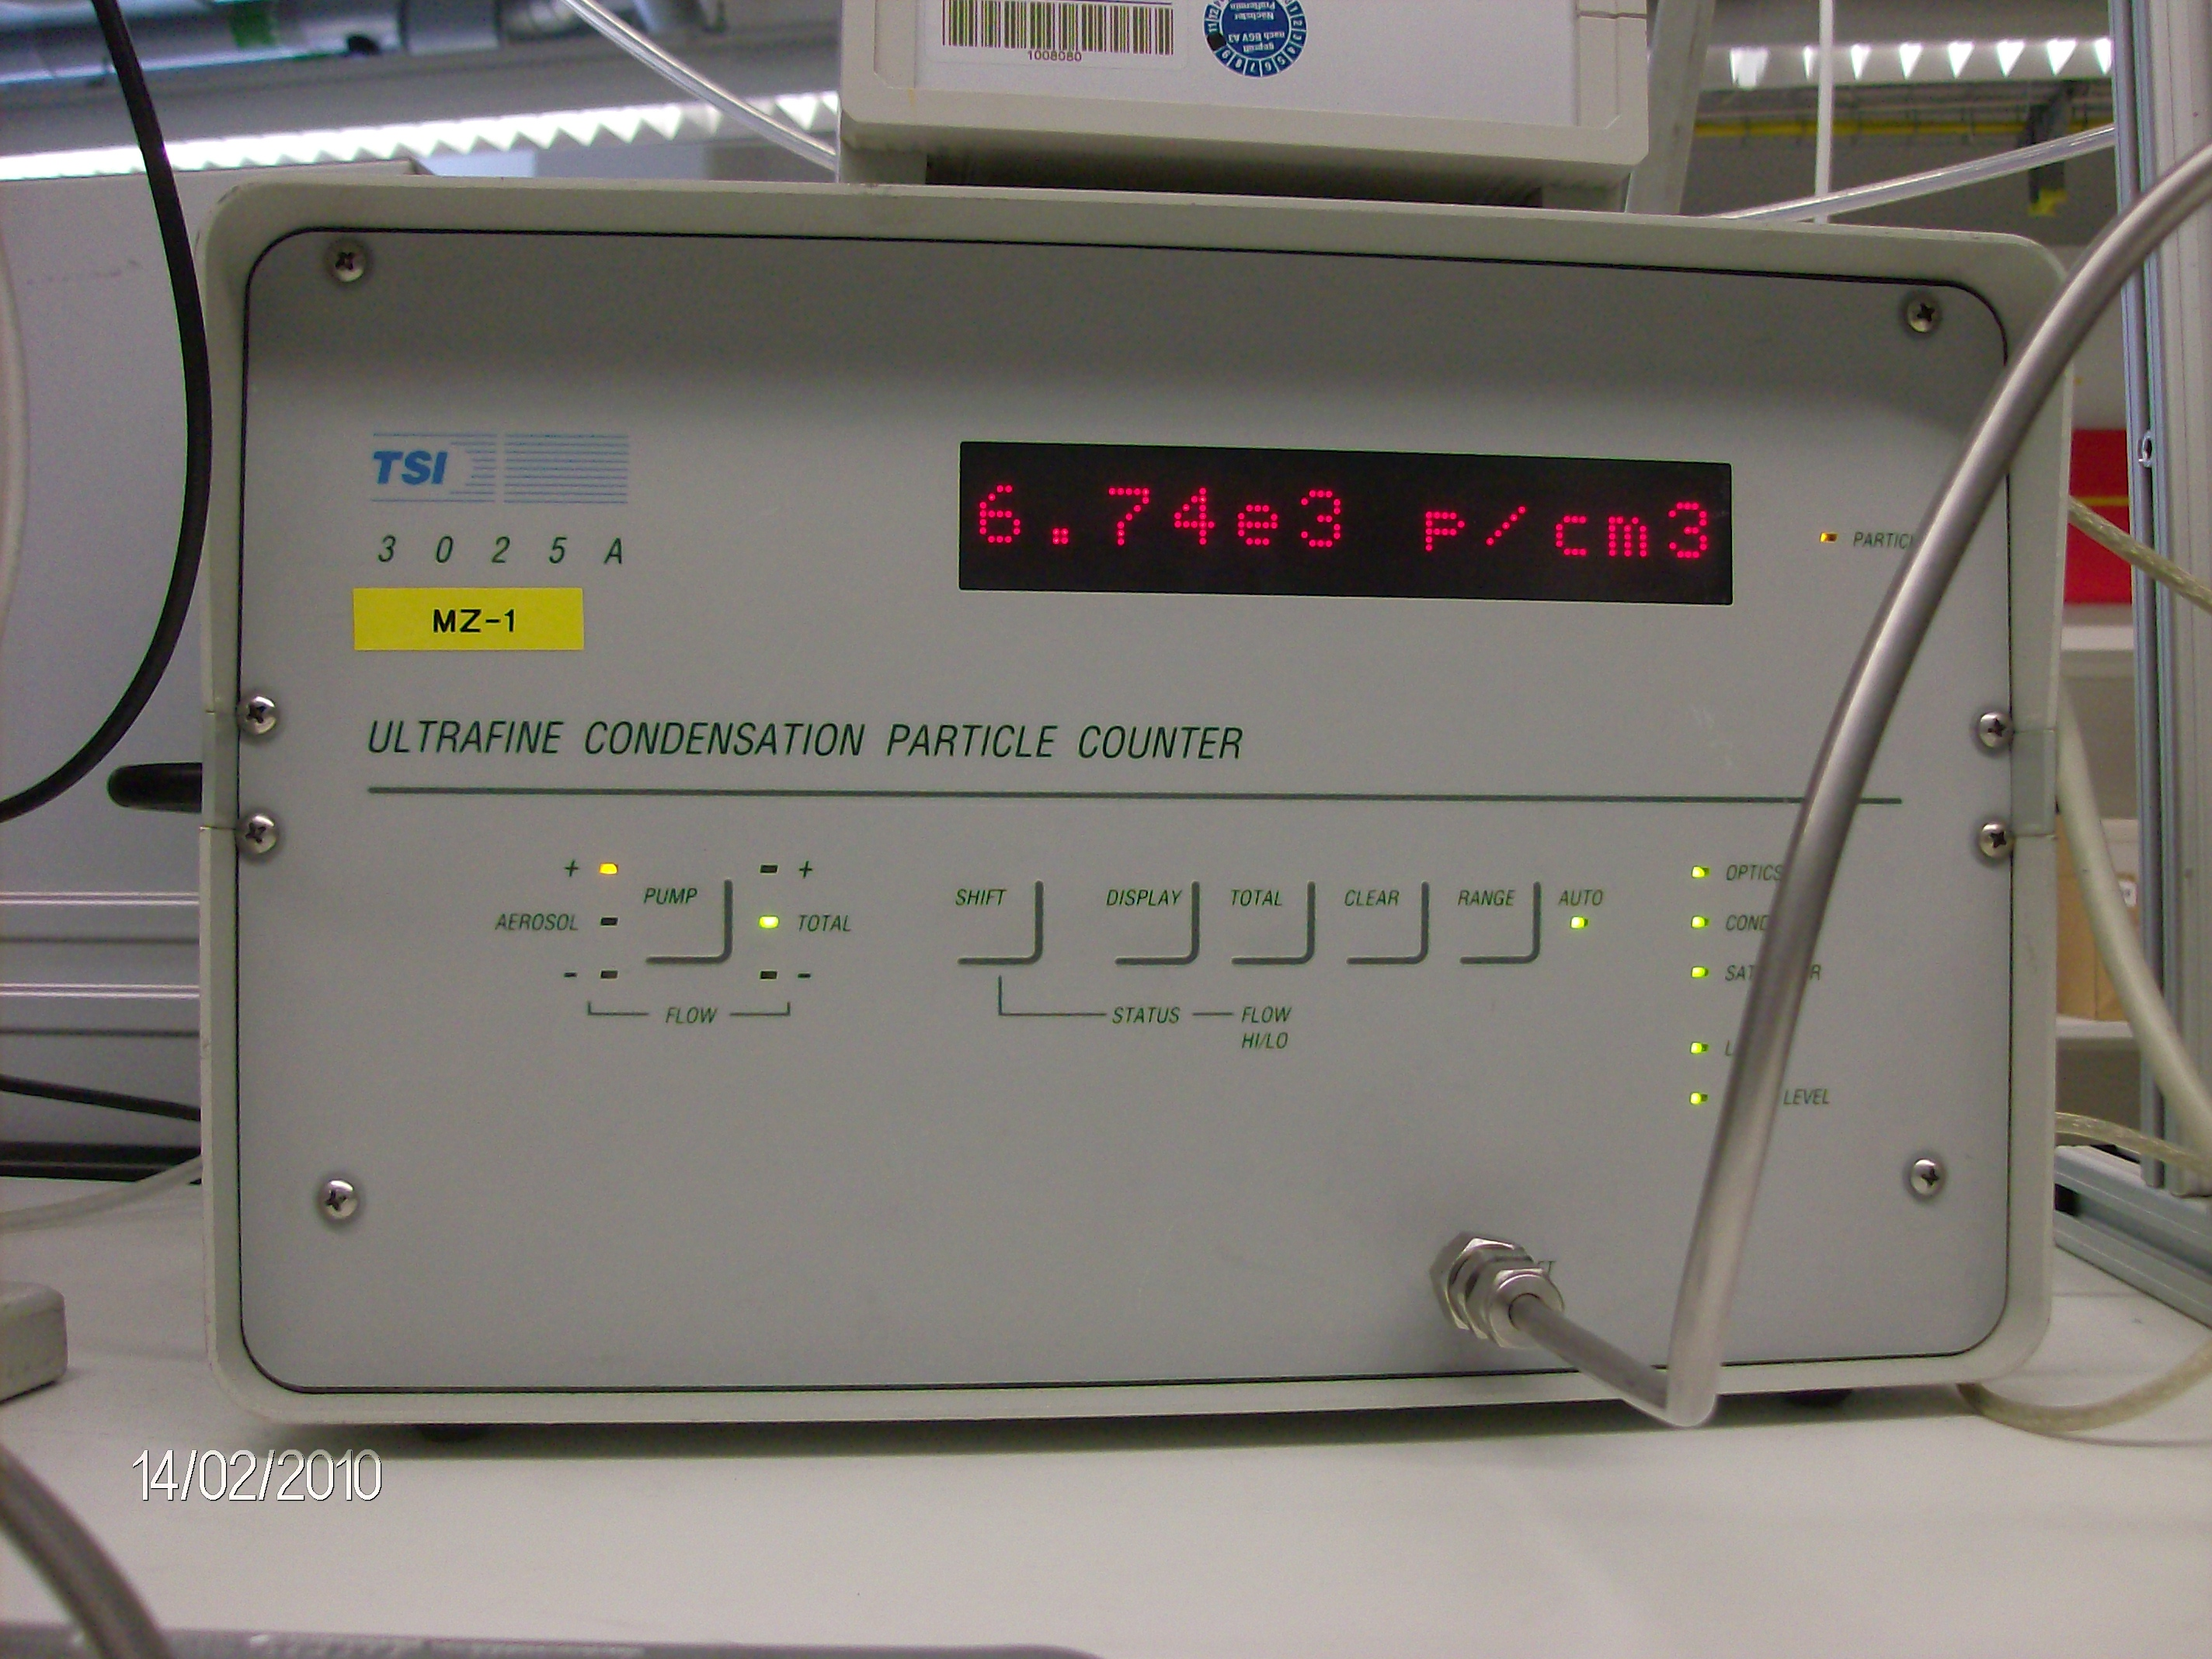
\includegraphics[scale=0.9]{eps/TSI3025CPC.eps}\\
\end{center}
\caption{\label{TSI3025CPC}\hspace{-0.1em} contador de part\'{\i}culas condens\'{a}veis  CPC (TSI 3025A).}
\end{figure}

\begin{figure}[hbt]
\begin{center}
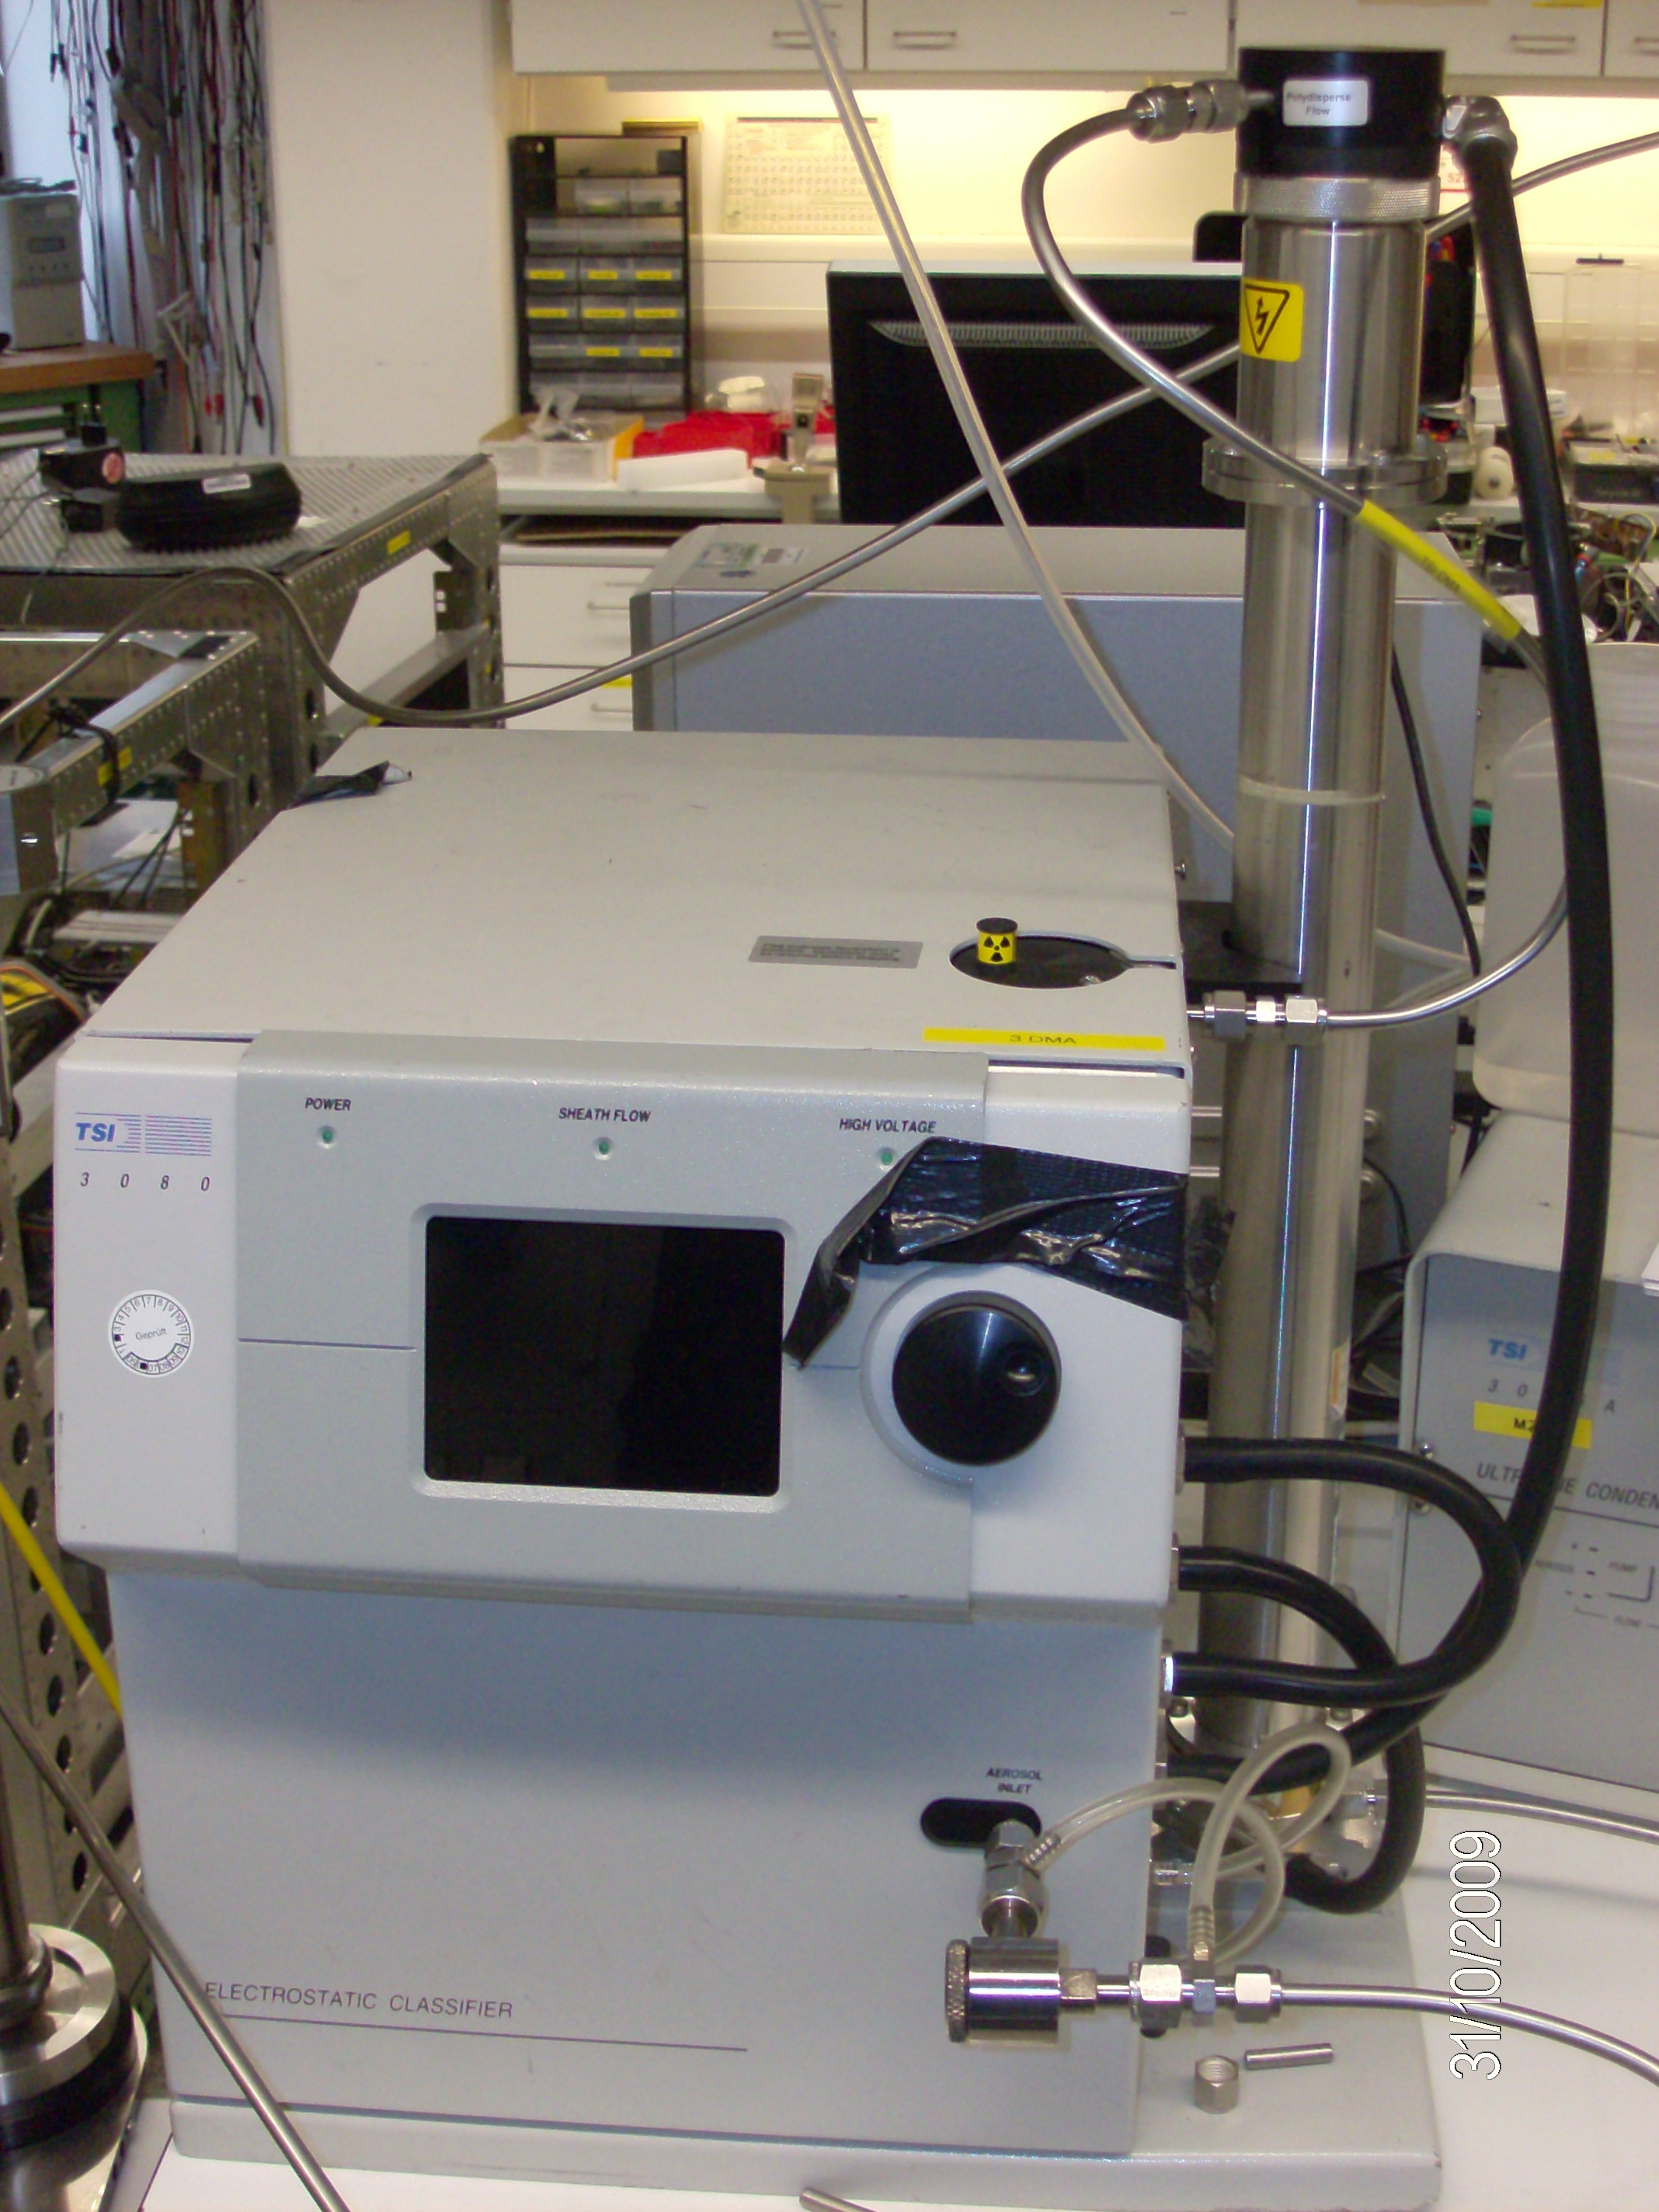
\includegraphics[scale=0.1]{eps/TSI3080CE.eps}\\
\end{center}
\caption{\label{TSI3080CE}\hspace{-0.1em} classificador eletrost\'{a}tico (TSI 3080).}
\end{figure}


\begin{figure}[hbt]
\begin{center}
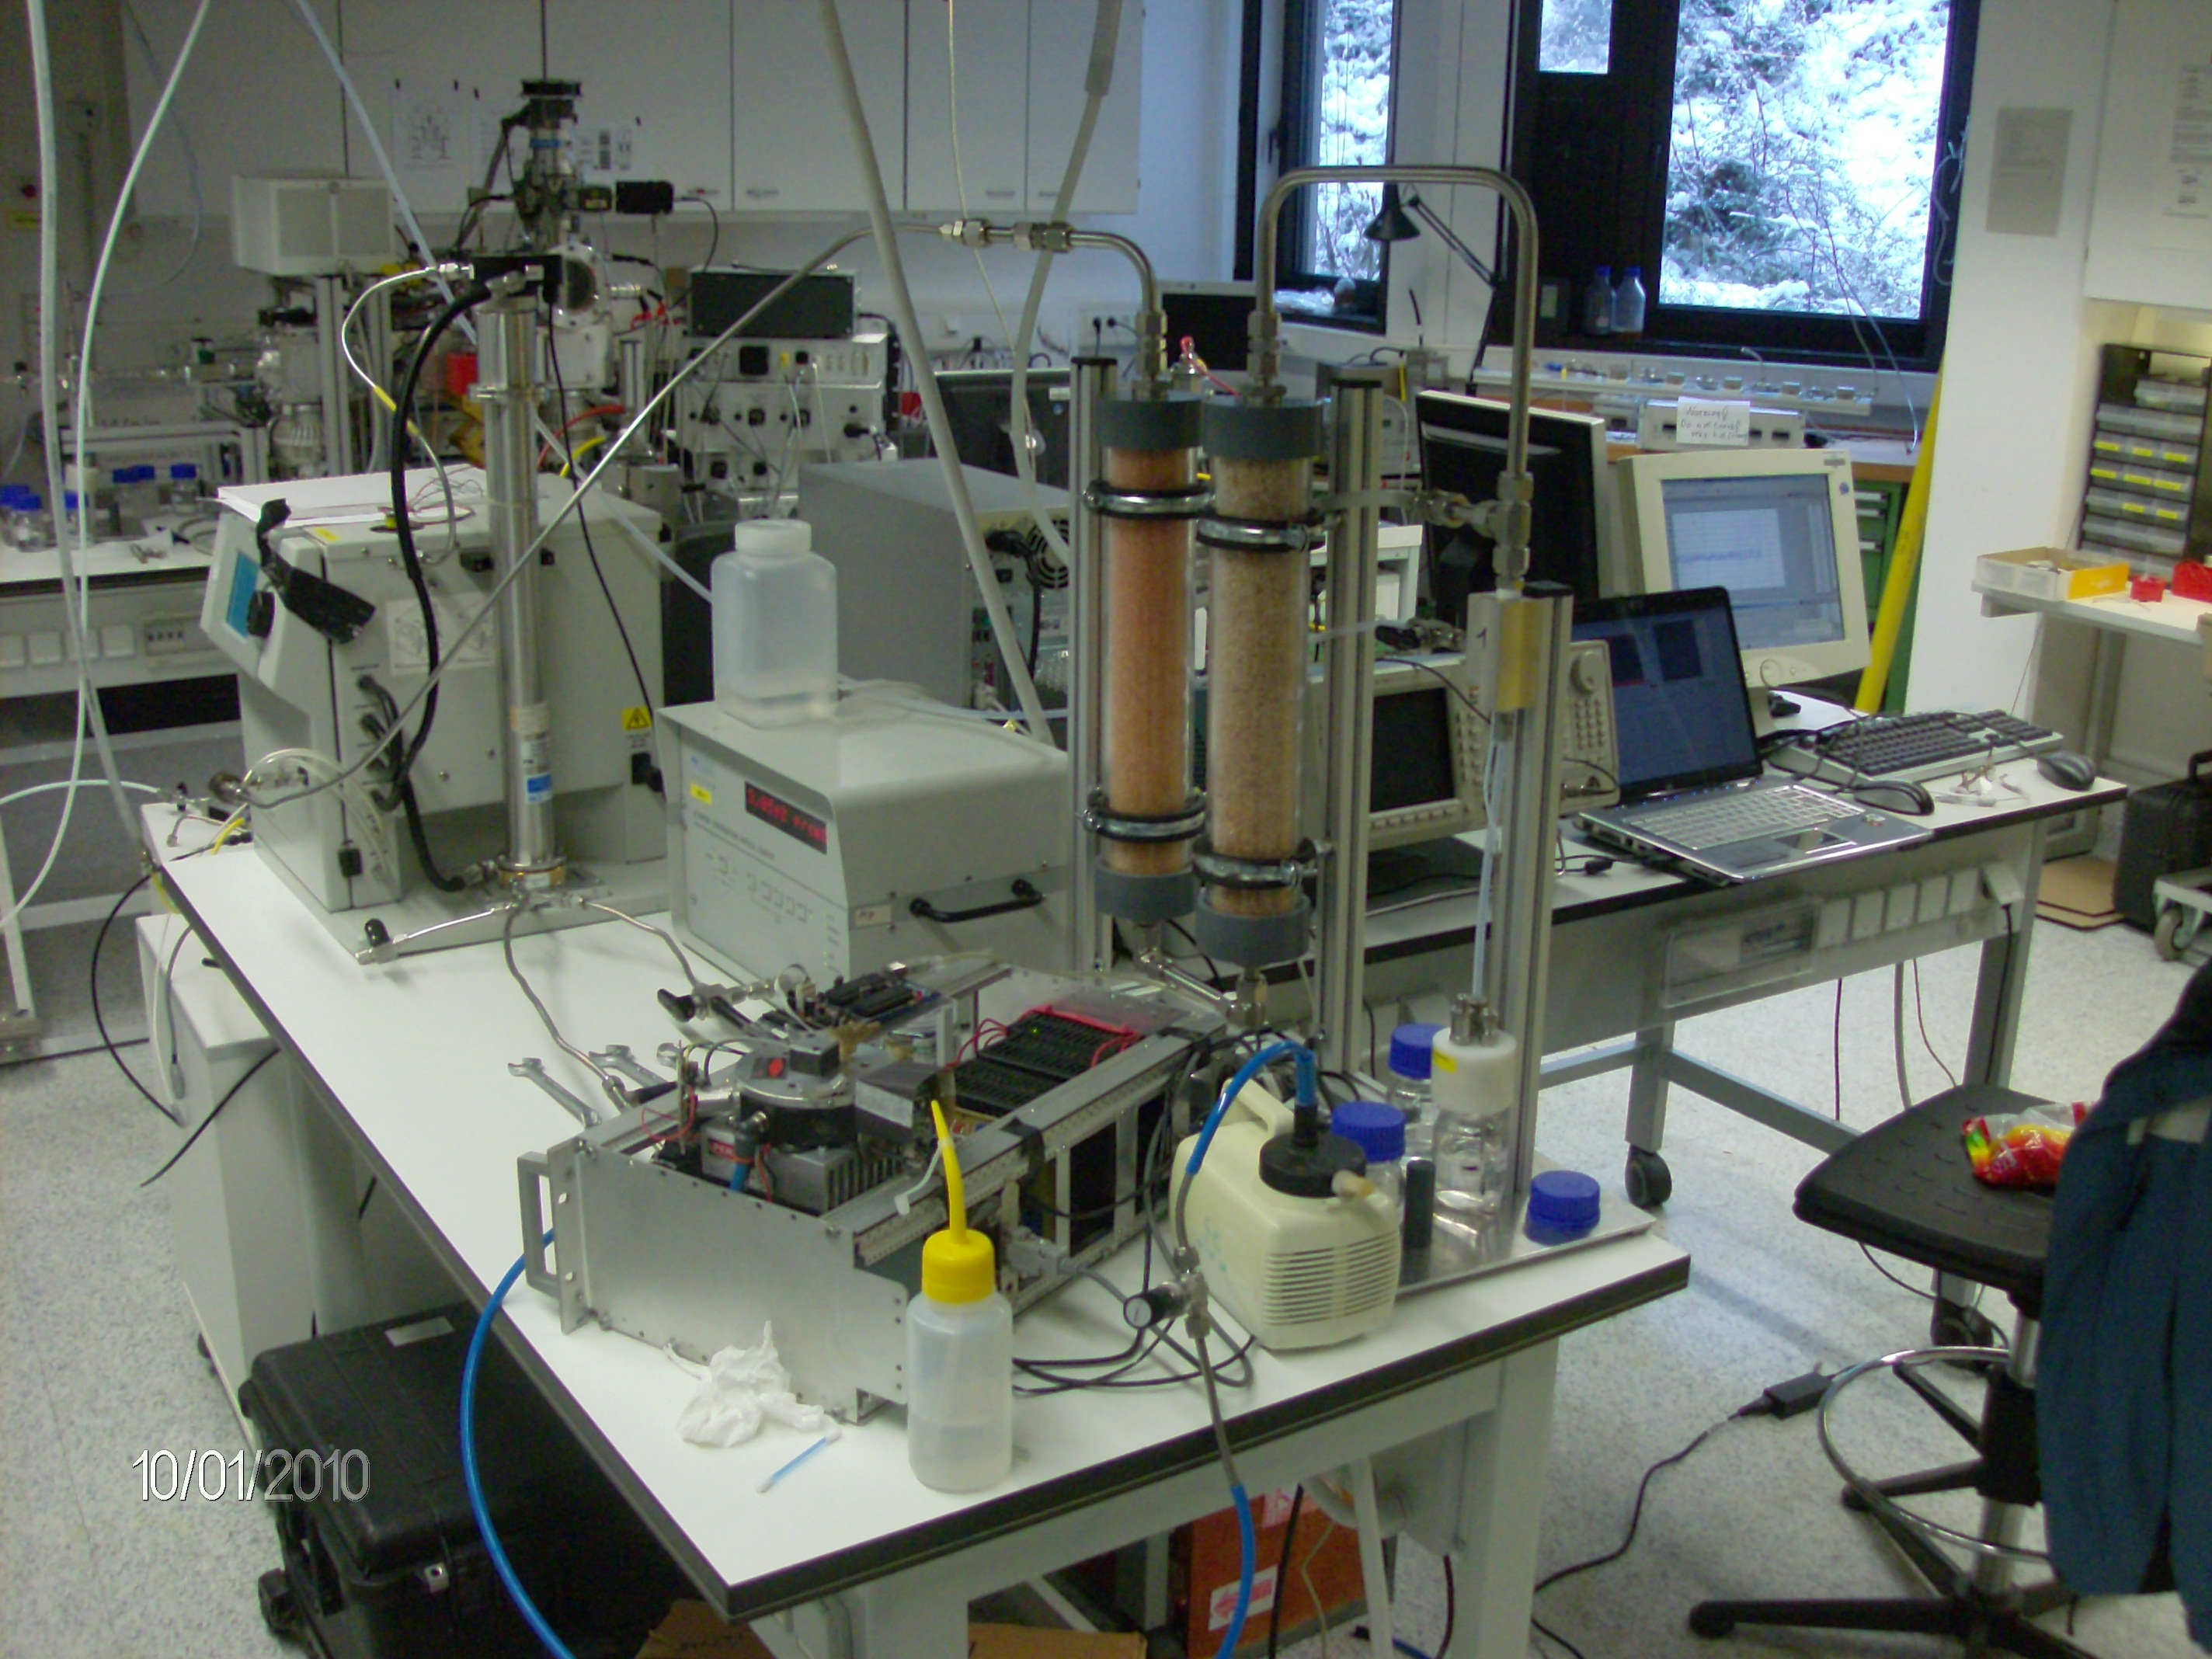
\includegraphics[scale=0.1]{eps/BANCADA_FOTO.eps}\\
\end{center}
\caption{\label{BANCADA_FOTO}\hspace{-0.1em} vista geral da bancada (TSI 3080).}
\end{figure}


\subsection{Prevenindo perda de part\'{\i}culas por deposi\c{c}\~{a}o eletrost\'{a}tica}
As medidas de aeross\'{o}is requerem um sistema de dutos para condu\c{c}\~{a}o destes aeross\'{o}is at\'{e} os mais variados instrumentos de medi\c{c}\~{a}o. Dependendo das caracter\'{\i}sticas f\'{\i}sicas dos aeross\'{o}is e dos dutos, diversos mecanismos de perda de part\'{\i}culas podem interferir nas medi\c{c}\~{o}es \cite{SL}. Uma destas causas chama-se de perda por deposi\c{c}\~{a}o eletrost\'{a}tica. Quando os aeross\'{o}is s\~{a}o produzidos em atomizadores, nebulizadores ou atrav\'{e}s de mecanismos naturais, alguns podem n\~{a}o estar eletricamente neutros. No caso destes aeross\'{o}is serem capturados pelos dutos de qualquer medidor de concentra\c{c}\~{a}o, pode ocorrer de algumas part\'{\i}culas ficarem retinas nos pr\'{o}prios dutos caso estes n\~{a}o sejam de material condutor e n\~{a}o estejam aterrados. Com o objetivo de verificar estas perdas, um experimento foi realizado e consistia em comparar a medida da concentra\c{c}\~{a}o realizada pelo CPC em 2 condi\c{c}\~{o}es: a primeira utilizando um duto coletor de 3 metros de pl\'{a}stico e a segunda utilizando um duto de a\c{c}o inox de mesmo comprimento. A medida foi realizada durante 50 segundos para cada caso. O resultado deste experimento mostrou que este efeito n\~{a}o pode ser negligenciado no caso de dutos longos, pois, a diferen\c{c}a chegou a 13\% na m\'{e}dia como \'{e} mostrado na Tabela \ref{perdas} e na Figura \ref{duto}.


\begin{table}[!htbp]
\centering \caption{\label{perdas} compara\c{c}\~{a}o entre concentra\c{c}\~{o}es medidas realizadas por dutos de a\c{c}o e pl\'{a}stico}
\begin{tabular}{ c | c  }
  \hline
  Tipo de duto & Concentra\c{c}\~{a}o m\'{e}dia\\
  \hline
  A\c{c}o & 2611\\
  Pl\'{a}stico & 2272\\
  \hline
  Diferen\c{c}a & 13 \% \\
  \hline
\end{tabular}\\
\end{table}



\begin{figure}[hbt]
\begin{center}
\includegraphics[scale=1.0]{eps/dutos.eps}\\
\end{center}
\caption{\label{duto}\hspace{-0.1em} perdas em fun\c{c}\~{a}o do tipo de duto. }
\end{figure}




